\documentclass[12pt, a4paper]{article}
\usepackage{amsmath, amsfonts, amssymb, amsthm, mathtools}

\usepackage{fontspec}
\setmainfont {Roboto}

\usepackage{unicode-math}
\setmathfont {Asana Math}

\DeclareMathOperator {\Var} {Var}

\usepackage{polyglossia}
\setdefaultlanguage {russian}
\setotherlanguage {english}

\usepackage{graphicx}


\begin {document}

\section{Факты о себе}

\begin{enumerate}
%Человек, который будет это проверять (если вдруг не только Филипп проверять будет), не воспринимай это всё серьёзно - это неудачная попытка самоиронии и чёрного юмора.
\item Ботан. \label{number_1}
\item Ещё раз ботан. \label{number_2}
\item Состою в неформальном клубе жёстких ботанов-общажников.\label{number_3}
\item Несмотря на пункты \ref{number_1}, \ref{number_2} и \ref{number_3}, не самый жёсткий ботан --- можно ещё жёстче. \label{number_4}
\item Несмотря на факт пункта \ref{number_4}, часто нахожусь на грани сумасшедствия. Единственное, почему ещё не рехнулся --- служба в храме.
\item Иногда встаю в ступор от вопроса: "Что делаешь в свободное время?", так как забываю, что значит "свободное время".
\item Так же ступорит вопрос про хобби.
\item В лично деле военкомата ступор предыдущего пункта решили просто: написали "увлечён учёбой".
\item Знаю, слава Богу, в чём смысл жизни. %реально знаю
\item Ходячая гремящая бочка --- считаю, что любое действие должно сопровождаться каким-то звуком, что дико бесит соседа, особенно в 5 утра.
\end{enumerate}


\section{Mоё фото}

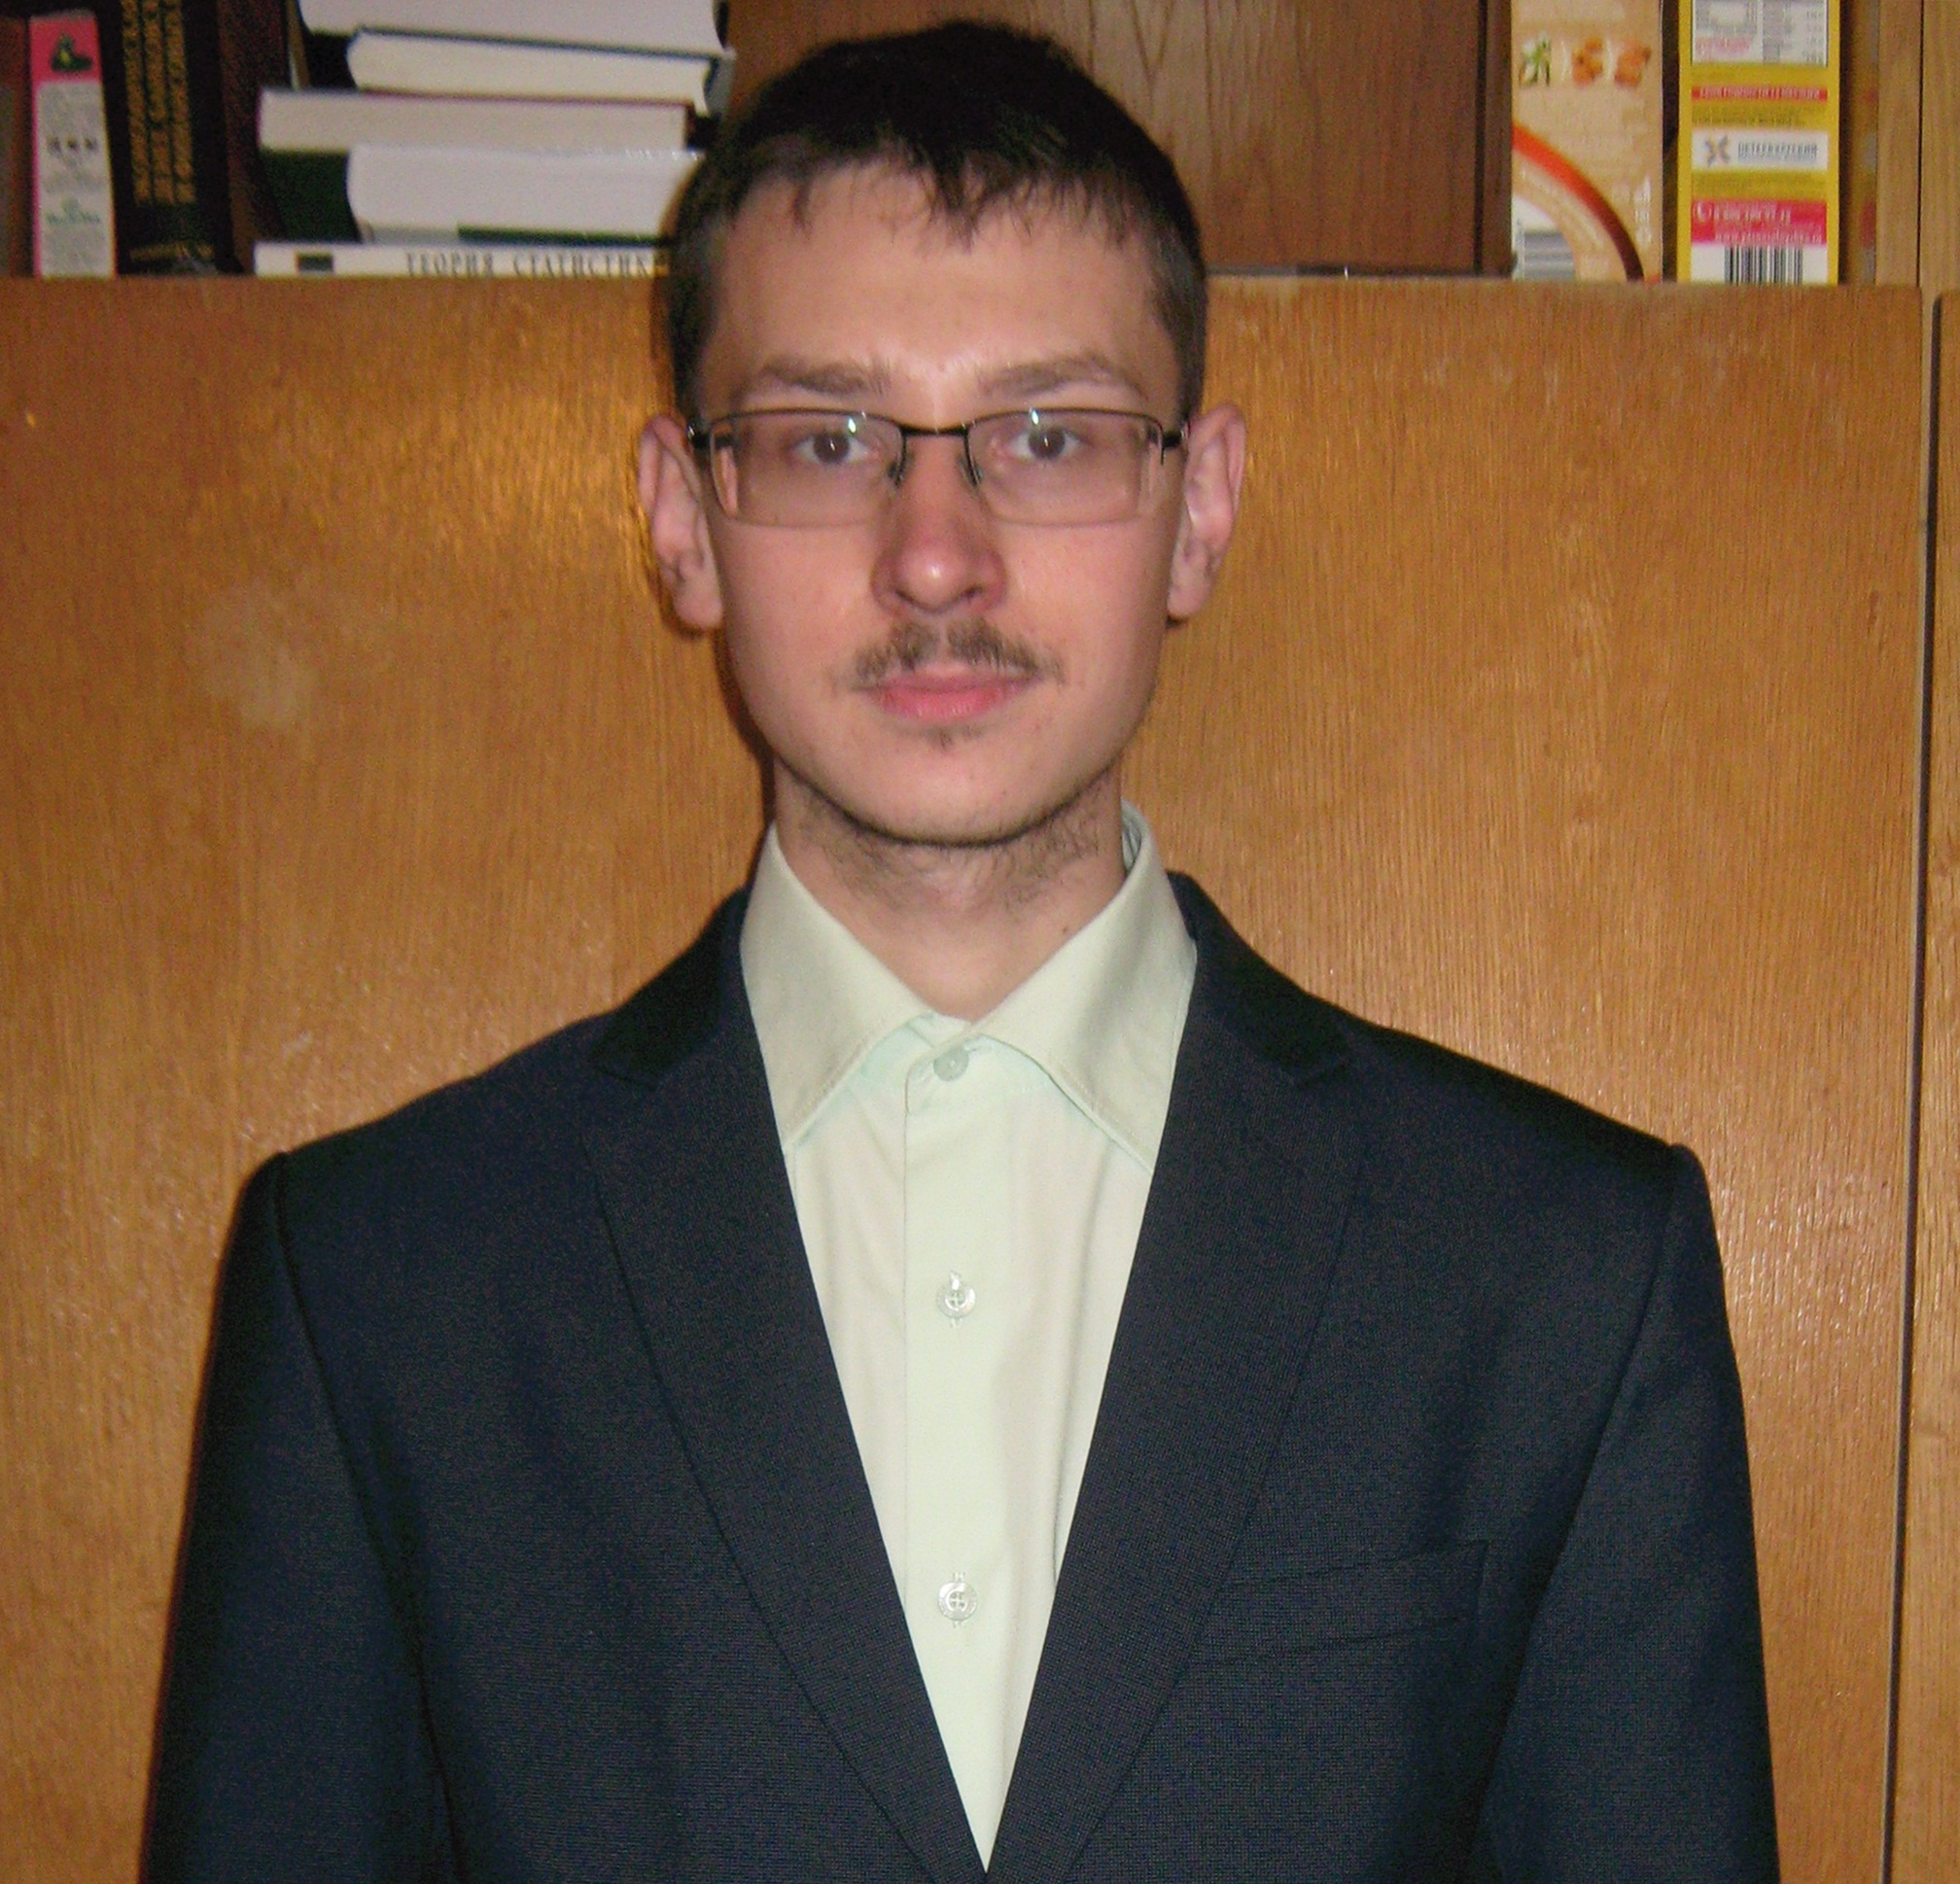
\includegraphics[scale=0.3]{I_03.jpg}


\section{Формулы 1}

\subsection{Любимые формулы}


\[
1+x+x^2+\ldots+x^n+\ldots = \sum_{n=0}^{\infty} x^n =
\frac{1}{1-x}, \quad |x|<1 \tag {\text {\ae}} \label{formula_1}
\]

\[
\lim_{x \to 0} \frac{\ln(1+x)}{x} = 1 
\tag {\text {\ae\ae}} \label{formula_2}
\]

\begin{multline*}
\text{Если } \varphi (y) = \int \limits_a^b f(x,y) dx, 
\text { то, при выполнении ряда условий, } \\
 \varphi'(y) = \int \limits_a^b \frac{\partial f}{\partial y} (x, y) dx
\tag {\text {\ae\ae\ae}} \label{formula_3}
\end{multline*}

\begin {multline*}
\lim_{x \to 4} \frac{3-\sqrt{5+x}}{1-\sqrt{5-x}} = \left[\frac{0}{0}\right]=
\lim_{x \to 4} \frac{(9-5-x)(1+\sqrt{5-x})}{(1-5+x)(3+\sqrt{5+x})}= \\
= -\lim_{x \to 4} \frac{(x-4)(1+\sqrt{5-x})}{(x-4)(3+\sqrt{5+x})}= -\lim_{x \to 4} \frac{1+\sqrt{5-x}}{3+\sqrt{5+x}}=-\frac{1}{3}
\tag {\text{\ae\ae\ae\ae}} \label{formula_4}
\end {multline*}

\[
 \begin{vmatrix}
  a_{1,1} & a_{1,2} & \cdots & a_{1,n} \\
  a_{2,1} & a_{2,2} & \cdots & a_{2,n} \\
  \vdots  & \vdots  & \ddots & \vdots  \\
  a_{n,1} & a_{n,2} & \cdots & a_{n,n}
 \end{vmatrix}
= \sum_{\substack {\text {по всем переста-}\\
\text {новкам } (i_1, \ldots, i_n)}} 
(-1)^{\text {знак } (i_1, \ldots, i_n)} \,\, 
a_{1 \, i_1} \cdot \ldots \cdot a_{n \, i_n}
\tag {\text {\ae\ae\ae\ae\ae}} \label{formula_5}
\]

\subsection{Нелюбимая формула}
\[
\sigma^2_{\hat{\beta}_1}= \frac{1}{n} \frac{\Var \, [(x_i-\mathsf{E}(x))\, u_i]}{(\Var \, (x_i))^2} \tag {\text {\ae\ae\ae\ae\ae\ae}}\label{formula_6}
\]

\section{Формулы 2}

$\quad$ Формула \eqref{formula_1} нравится, потому что позволяет получать разные прикольные результаты, особенно в финансах. \eqref{formula_2} даёт возможность заменить дробь $\displaystyle \frac{x_2-x_1}{x_1}$ на разность
$\ln x_2 - \ln x_1$, что отлично помогает в метрике. Формула \eqref{formula_3} (вернее, это даже не формула, а кусок теоремы) говорит, что иногда можно поменять местами производную и интеграл, что само по себе прикольно. \eqref{formula_4} опять-таки не формула, а пример, но зато классный: он иллюстрирует тот факт, что, в математике если знаешь, что делать, то любую самую жуткую, отвратительную громозеку можно свернуть до маленькой, приятной вещи, которая считается на раз-два. 

 Формула \eqref{formula_5} просто шедевр! Взять откуда-то в матрице эту фигню (которая считается по такой дикой формуле), придумать кучу способов, как эту дрянь проще считать, и потом обнаружить, что эта фигня позволяет определить кучу классных свойств матрицы - это гениально!

 \eqref{formula_6} просто подстава от Стока-Ватсона и Турунцевой Марины Юрьевны. Заставлять учить эту и подобные гадости, когда есть классная формула в матричном виде, которая позволяет найти $\sigma^2$ для любой $\hat{\beta}$!
\end{document}